\documentclass[12pt,a4paper]{article}

\usepackage[utf8]{inputenc}
\usepackage[T2A]{fontenc}
\usepackage[ukrainian]{babel}
\usepackage{geometry}
\geometry{
    left=2cm,
    right=2cm,
    top=2cm,
    bottom=2cm
}

\usepackage[table]{xcolor}
\usepackage{amsmath}
\usepackage{graphicx}
\usepackage{subcaption}
\usepackage{multirow}
\usepackage{makecell}
\usepackage{pdflscape}
\usepackage{array}
\newcolumntype{C}[1]{>{\centering\arraybackslash}m{#1}}

\usepackage{minted}

\usemintedstyle{vs}
\setminted{linenos, breaklines, frame=single, fontsize=\small}

\RecustomVerbatimCommand{\VerbatimInput}{VerbatimInput}{
    breaklines=true,
    breaksymbolleft={}
}

\usepackage[
  unicode,
  pdftitle={ІО-41, Давидчук А.М., Цифрова схемотехніка, Лабораторна робота №4},
  pdfauthor={Давидчук Артем},
  pdfsubject={Цифрова схемотехніка}
]{hyperref}

\begin{document}

    \begin{titlepage}

        \begin{center}
\includegraphics[width=0.7\textwidth]{../../../TITLES/letterhead.png}\end{center}

        \begin{center}
            \large Національний технічний університет України\\
            «Київський політехнічний інститут імені Ігоря Сікорського»\\[1em]
            Факультет інформатики та обчислювальної техніки\\
            Кафедра обчислювальної техніки
        \end{center}

        \vfill

        \begin{center}
            \textbf{\LARGE Цифрова схемотехніка}\\[2em]
            \textbf{\Large Лабораторна робота №4}\\[0.5em]
            «Розроблення схем комбінаційної логіки»
        \end{center}

        \vfill

        \begin{flushright}
            Виконав: студент 2 курсу ФІОТ, гр. ІО-41\\
            \textit{Давидчук А. М.}\\
            Залікова книжка № 4106\\[1em]
            Перевірив: \textit{Нікольський С.\,С.}
        \end{flushright}

        \vfill

        \begin{center}Київ --- 2026\end{center}

    \end{titlepage}

    \noindent
    \textbf{\underline{Тема:}} «Розроблення схем комбінаційної логіки».

    \vspace{1em}

    \begin{center} \textbf{\Large Хід роботи} \end{center}

    Мій номер залікової книжки: 4106, що у двіковому вигляді є 0001 0000 0000 1010.
    Звідси $h_7 = 0, h_6 = 0, h_5 = 0, h_4 = 1, h_3 = 0, h_2 = 1, h_1 = 0$.
    Звідси маю такий варіант:

    \begin{table}[h]
        \centering
        \renewcommand{\arraystretch}{1.3}
        \begin{tabular}{|cccccc|}
        \hline
        $0$ & $0$ & $1$ & $0$ & $1$ & $0$ \\
        \hline
        $h_6$ & $h_5$ & $h_4$ & $h_3$ & $h_2$ & $h_1$ \\
        \hline
        \end{tabular}
        \caption{Таблиця значеннь розрядів}
    \end{table}

    \noindent
    Параметри перемикальної функції:

    \begin{table}[h]
        \centering

        \begin{minipage}[t]{0.48\textwidth}
        \centering
        \renewcommand{\arraystretch}{1.2}
        \begin{tabular}{|c|c|}
        \hline
        $x_3\;\;x_2\;\;x_1$ & $f_4$ \\
        \hline
        $0\;\;0\;\;0$ & $0$ \\
        $0\;\;0\;\;1$ & $0$ \\
        $0\;\;1\;\;0$ & $0$ \\
        $0\;\;1\;\;1$ & $1$ \\
        $1\;\;0\;\;0$ & $0$ \\
        $1\;\;0\;\;1$ & $1$ \\
        $1\;\;1\;\;0$ & $0$ \\
        $1\;\;1\;\;1$ & $1$ \\
        \hline
        \end{tabular}
        \caption{Таблиця істинності функції $f_4$}
        \end{minipage}
        \hfill
        \begin{minipage}[t]{0.48\textwidth}
        \centering
        \renewcommand{\arraystretch}{1.4}
        \begin{tabular}{|c|c|}
        \hline
        \textbf{$h_1\;h_5\;h_2$} & \textbf{Логічні елементи} \\
        \hline
        $0\;0\;0$ & I-НЕ, I \\
        \hline
        \rowcolor{yellow!35}
        $0\;0\;1$ & I-НЕ \\
        \hline
        $0\;1\;0$ & АБО, I, НЕ \\
        \hline
        $0\;1\;1$ & I, АБО, НЕ \\
        \hline
        $1\;0\;0$ & АБО-НЕ, АБО \\
        \hline
        $1\;0\;1$ & I-НЕ, АБО \\
        \hline
        $1\;1\;0$ & АБО-НЕ, I-НЕ \\
        \hline
        $1\;1\;1$ & I, АБО-НЕ \\
        \hline
        \end{tabular}
        \caption{Елементний базис перемикальної функції}
        \end{minipage}

    \end{table}

    Звідси реалізую функцію $f_4$ у єдиному елементному базисі 2І-НЕ\slash 2І-НЕ (нехай використовуватиму саме 2І-НЕ елемент). 2І-НЕ\slash 2І-НЕ можна отримати із МДНФ функції $f_4$, додати два заперечення над усім виразом, а потім за законом де Моргана дійти до потрібної нормальної форми, а потім до операційної.

    \vspace{1em}

    ДДНФ функції $f_4$:

    \[
    f_4 (\text{ДДНФ}) = \overline{x_3} x_2 x_1 \vee x_3 \overline{x_2} x_1 \vee x_3 x_2 x_1
    \]

    \newpage

    І зробимо мінімізацію за допомогою діаграми Вейча:

    \begin{figure}[h]
        \centering
        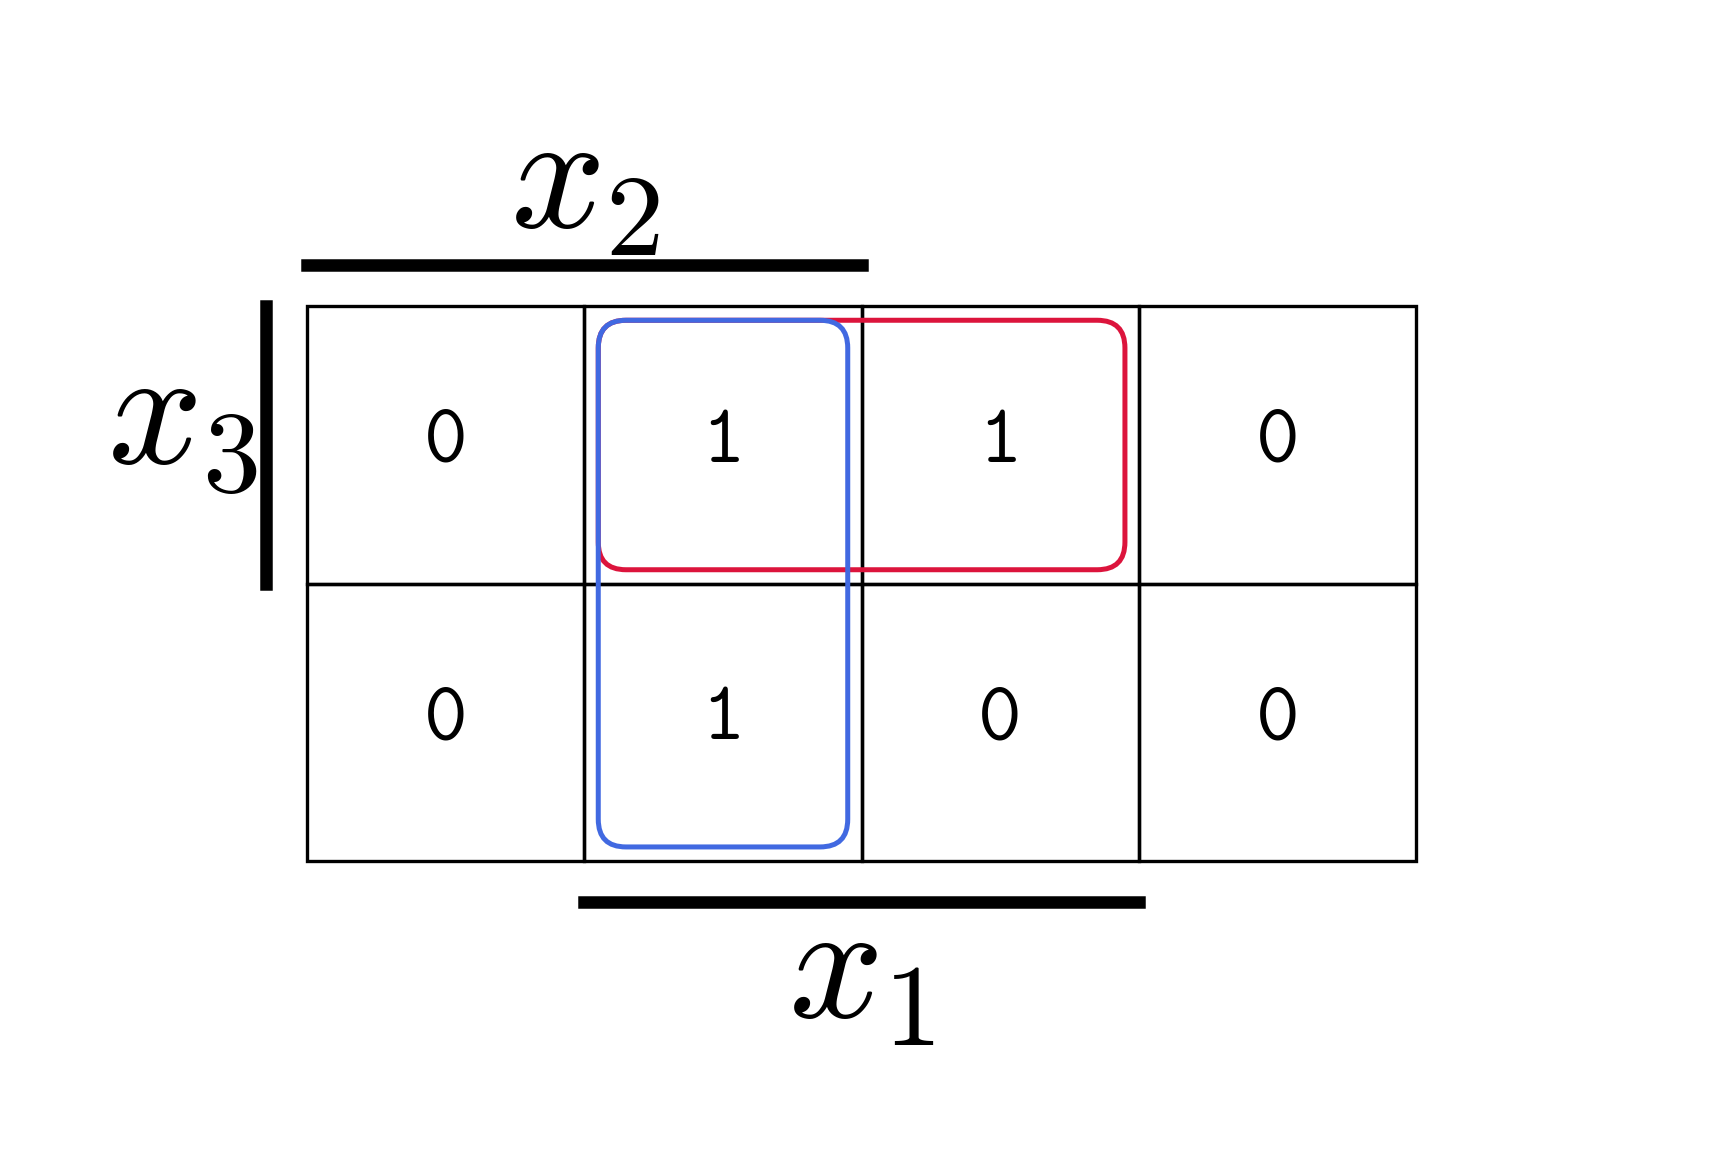
\includegraphics[width=0.5\textwidth]{media/minimized_f.png}
        \caption{Діаграма Вейча}
    \end{figure}

    \noindent
    Звідси МДНФ вираз для функції $f_4$:

    \vspace{0.5em}

    $f_4 (\text{МДНФ}) = x_2 x_1 \vee x_3 x_1$

    \vspace{1em}

    \noindent
    Тепер переведемо до нормальної форми:

    \vspace{0.5em}

    $f_4 (\text{МДНФ}) = \overline{\overline{f_4 (\text{МДНФ})}} = \overline{\overline{x_2 x_1 \vee x_3 x_1}} = \overline{\overline{x_2 x_1} \wedge \overline{x_3 x_1}}$

    \vspace{1em}

    \noindent
    А також визначимо операторну форму для елементів 2І-НЕ:

    \vspace{0.5em}

    $F_4 = \overline{\overline{x_2 x_1} \wedge \overline{x_3 x_1}}$

    \vspace{1em}

    \noindent
    Тепер запишемо код, який реалізує дану комбінаційну схему мовою Verilog:

    \begin{minted}{verilog}
module F4(x1, x2, x3, f);
  input x1, x2, x3;
  output f;
  assign f = ~(~(x2 & x1) & ~(x3 & x1));
endmodule
    \end{minted}

    \noindent
    Та виконуваний файл Stim.do:

    \begin{minted}{text}
force x1 2#0 0ns, 2#1 50ns, 2#0 100ns, 2#1 150ns, 2#0 200ns, 2#1 250ns, 2#0 300ns, 2#1 350ns;
force x2 2#0 0ns, 2#1 100ns, 2#0 200ns, 2#1 300ns;
force x3 2#0 0ns, 2#1 200ns;
    \end{minted}

    \newpage

    \noindent
    І наведемо часову діаграму функції $f$:

    \begin{figure}[h]
        \centering
        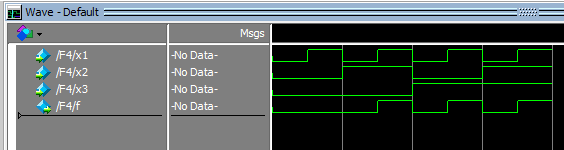
\includegraphics[width=\textwidth]{media/diag.png}
        \caption{Часова діаграма}
    \end{figure}

    \noindent
    Як можна спостерігати, значення функції $f$ набуває одиниці лише в 3 випадках:

    \begin{itemize}
        \item Коли $x_3 = 0, x_2 = 1, x_1 = 1$
        \item Коли $x_3 = 1, x_2 = 0, x_1 = 1$
        \item Коли $x_3 = 1, x_2 = 1, x_1 = 1$
    \end{itemize}

    Тобто співпадає із таблицею істинності, що свідчить про правильний синтез та симуляцію цієї комбінаційної схеми.

    \vspace{1em}

    \noindent
    Загальне фото вікна програми ModelSim:

    \begin{figure}[h]
        \centering
        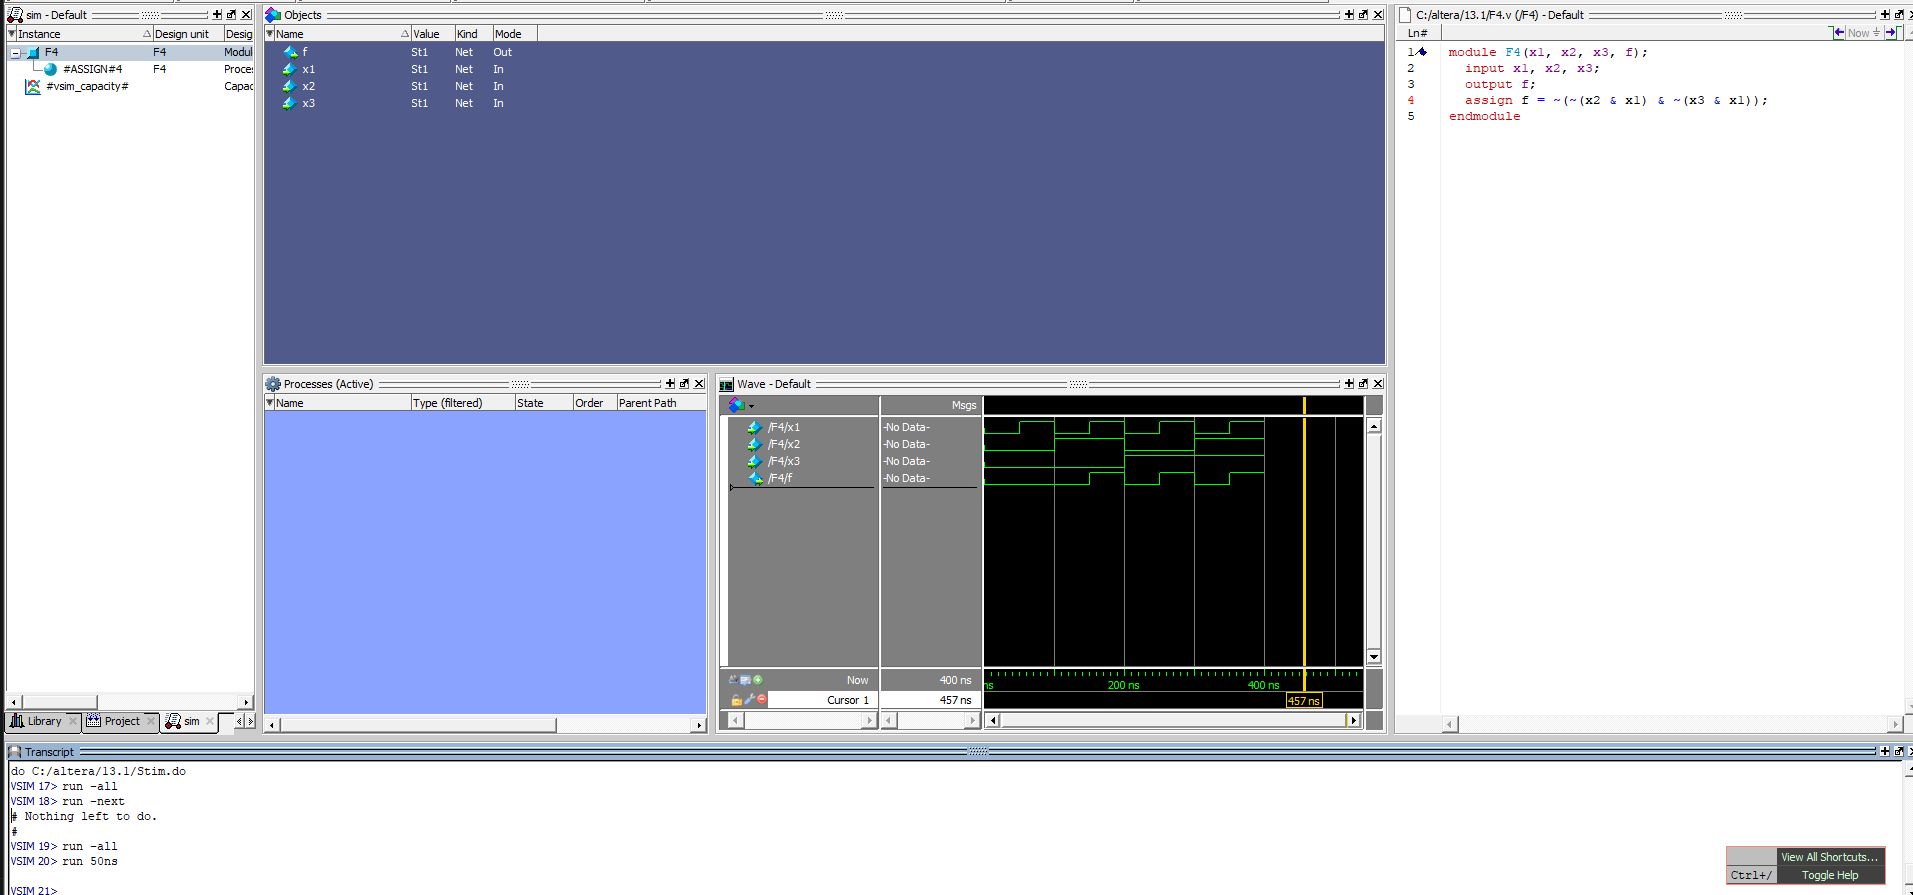
\includegraphics[width=\textwidth]{media/all.png}
        \caption{Загальний вигляд}
    \end{figure}

    \begin{center} \textbf{\Large Висновок} \end{center}

    У ході виконання лабораторної роботи було розроблено комбінаційну логічну схему для функції $f_4$ відповідно до заданого варіанта. На основі таблиці істинності було побудовано ДДНФ функції, після чого за допомогою діаграми Вейча виконано її мінімізацію та отримано МДНФ $f_4 = x_2x_1 \vee x_3x_1$. Далі функцію було перетворено до форми, зручної для реалізації в єдиному елементному базисі 2І-НЕ, та реалізовано мовою Verilog.

    За допомогою ModelSim проведено симуляцію роботи схеми, побудовано часову діаграму та перевірено відповідність отриманих результатів таблиці істинності. Отже, у роботі було успішно виконано синтез, програмну реалізацію та верифікацію комбінаційної логічної схеми, а також закріплено практичні навички мінімізації логічних функцій і моделювання цифрових пристроїв.

\end{document}